\documentclass[convert = false, tikz]{standalone}
\usepackage[utf8]{inputenc}
\usepackage{tikz}
\usetikzlibrary{automata, positioning, arrows}
 
\usepackage{../../../../style_automata}

\begin{document}
    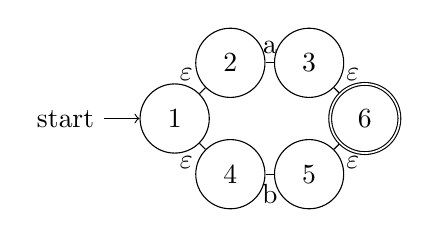
\begin{tikzpicture}
        \node[state, initial] (1) {$1$};
        \node[state, above right of=1] (2) {$2$};
        \node[state, right of=2] (3) {$3$};
        \node[state, below right of=1] (4) {$4$};
        \node[state, right of=4] (5) {$5$};
        \node[state, accepting, below right of=3] (6) {$6$};
        \draw (1) edge[above left] node{\(\varepsilon\)} (2)
        (2) edge[above] node{a} (3)
        (1) edge[below left] node{\(\varepsilon\)} (4)
        (4) edge[below] node{b} (5)
        (3) edge[above right] node{\(\varepsilon\)} (6)
        (5) edge[below right] node{\(\varepsilon\)} (6);
    \end{tikzpicture}
\end{document}